%!TEX root = ../RfCPN.tex


\modHeadchapter[loColumn,lof]{\WorkTotalLength および振分けの幾何\label{chap:ACallocation}\vphantom{\ref{chap:ACallocation}}}
\Alocation の長さ(\textbf{\AlocationLength})は、トップ側とボトム側では一般に異なる。
しかし、加工をする際には\JigCenter に対して両者の長さの差が小さいほうが一般的には好都合である。
そうした場合の対処法として、ここでは以下のような2つの方法を考える。
\begin{enumerate}
\item
適当な厚さの\textbf{\Spacer}を\index{ワークと\yomiJig のせってん@ワークと\nameJig の接点}ワークと\nameJig の接点に取り付けることで、双方の\AlocationLength を調節
\item
適当な角度に\Table を傾けることで、双方の\AlocationLength を調節
\end{enumerate}
このとき、\index{ワーク}ワークがどのように移動するかを考える。

基本的な考え方として、\textbf{\CenterCurvatureRadius}$R_\mathrm c$の円の中心を原点として$\Omega$だけ回転し、次に\index{ワーク}ワークとの(\Spacer を装着していない側の)接点を中心に$-\theta$だけ回転したと考えることができる。
なお、ここでは話の簡単化のため、もとの\Alocation ではトップ側より\BottomAlocationLength のほうが長いものとする。



%%%%%%%%%%%%%%%%%%%%%%%%%%%%%%%%%%%%%%%%%%%%%%%%%%%%%%%%%%
%% section 17.01 %%%%%%%%%%%%%%%%%%%%%%%%%%%%%%%%%%%%%%%%%
%%%%%%%%%%%%%%%%%%%%%%%%%%%%%%%%%%%%%%%%%%%%%%%%%%%%%%%%%%
\modHeadsection{\Jig の接点部が点の場合}
まずは簡単のため、\Jig の\index{ワーク}ワークとの接点部(\pageautoref{fig:mouldOnComplexPlane1}のU$_\mathrm T$, U$_\mathrm B$)は点であるとして考える。
%%%%%%%%%%%%%%%%%%%%%%%%%%%%%%%%%%%%%%%%%%%%%%%%%%%%%%%%%%
%% figure %%%%%%%%%%%%%%%%%%%%%%%%%%%%%%%%%%%%%%%%%%%%%%%%
%%%%%%%%%%%%%%%%%%%%%%%%%%%%%%%%%%%%%%%%%%%%%%%%%%%%%%%%%%
\begin{figure}[p]
\centering%
\begin{Figlandscape}
\captionsetup{width=.75\textheight}
\begin{adjustbox}{%
  addcode={\begin{minipage}{\textheight}\centering}{%
    \captionof{figure}[\CurvatureCenter Oを\index{げんてんO@原点O}原点とした\index{ふくそへいめん@複素平面}複素平面上の\index{ワーク}ワーク]{%
      \CurvatureCenter Oを\index{げんてんO@原点O}原点とした\index{ふくそへいめん@複素平面}複素平面上の\index{ワーク}\newline
      T$_\mathrm o$, T$_\mathrm i$, B$_\mathrm o$, B$_\mathrm i$, U$_\mathrm T$, U$_\mathrm B$は点、%
      $R_\mathrm c$, $R_\mathrm o$, $R_\mathrm i$, $f_\mathrm T$, $f_\mathrm B$, $l$は長さ、%
      $\alpha_{\mathrm T_\mathrm o}$, $\alpha_{\mathrm T_\mathrm i}$, $\alpha_{\mathrm U_\mathrm B}$は角度を示す。%
      \label{fig:mouldOnComplexPlane1}%
    }%
    \end{minipage}%
  },
  rotate=90,
  max width=\textwidth,
  max height=\textheight,
  keepaspectratio}
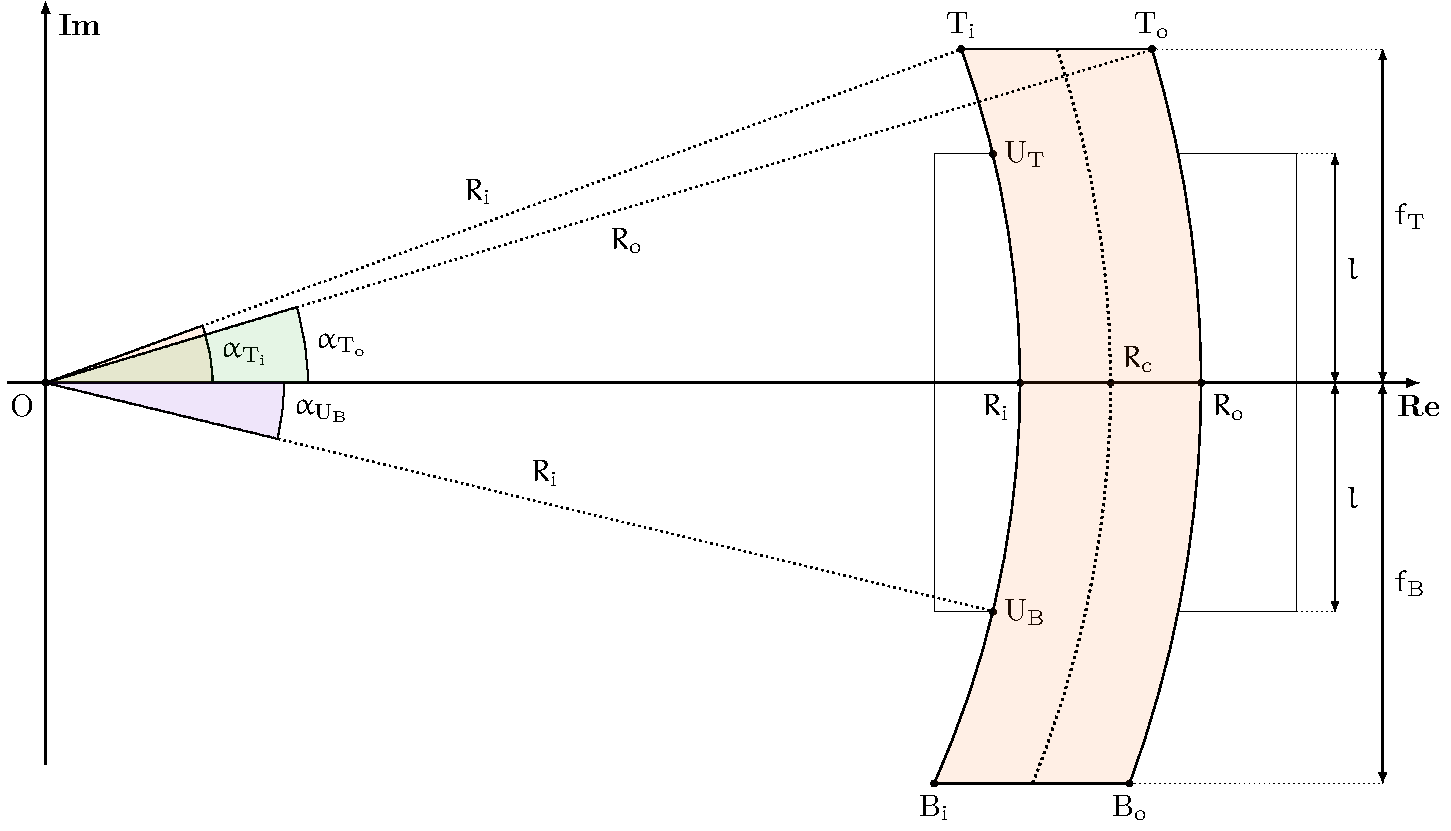
\includegraphics{RfCPN_p05_pictures/mouldoverall.pdf}
\end{adjustbox}
\end{Figlandscape}%
\end{figure}
%%%%%%%%%%%%%%%%%%%%%%%%%%%%%%%%%%%%%%%%%%%%%%%%%%%%%%%%%%
%%%%%%%%%%%%%%%%%%%%%%%%%%%%%%%%%%%%%%%%%%%%%%%%%%%%%%%%%%
%%%%%%%%%%%%%%%%%%%%%%%%%%%%%%%%%%%%%%%%%%%%%%%%%%%%%%%%%%


%%%%%%%%%%%%%%%%%%%%%%%%%%%%%%%%%%%%%%%%%%%%%%%%%%%%%%%%%%
%% subsection 17.01.01 %%%%%%%%%%%%%%%%%%%%%%%%%%%%%%%%%%%
%%%%%%%%%%%%%%%%%%%%%%%%%%%%%%%%%%%%%%%%%%%%%%%%%%%%%%%%%%
\subsection{\Spacer を用いた\ReAlocation}
\CurvatureCenter\expandafterindex{O(\yomiCurvatureCenter)@O(\nameCurvatureCenter)}Oを\index{げんてんO@原点O}原点とした\index{ふくそへいめん@複素平面}複素平面を考える
%% footnote %%%%%%%%%%%%%%%%%%%%%
\footnote{ここでは$0 < R_\mathrm c < \infty$ ($0 < \nicefrac1{R_\mathrm c} < \infty$)としている。
$R_\mathrm c \to \infty$ ($\nicefrac1{R_\mathrm c} \to 0$)の場合、すなわち\index{わんきょくのないモールド@湾曲のないモールド}湾曲のないまっすぐなモールドの場合は、別途考える必要がある。}。
%%%%%%%%%%%%%%%%%%%%%%%%%%%%%%%%%
このとき、\pageautoref{fig:mouldOnComplexPlane1}のように、$R_\mathrm c$, $R_\mathrm i$, $R_\mathrm o$, $f_\mathrm T$, $f_\mathrm B$, $l$, $\alpha_{\mathrm T_\mathrm i}$, $\alpha_{\mathrm T_\mathrm o}$, $\alpha_{\mathrm U_\mathrm B}$をとると、
\begin{subequations}
%% label{eq:constraintUpoint1}
%% label{eq:constraintUpoint2}
\begin{gather}
  \label{eq:constraintUpoint1}
  R_\mathrm o - R_\mathrm c = R_\mathrm c - R_\mathrm i = \frac{W_x}2~, \qquad
  \Im\ab(R_\mathrm oe^{i\alpha_{\mathrm T_\mathrm o}} - R_\mathrm ie^{i\alpha_{\mathrm T_\mathrm i}})
  = 0~,\\
  \label{eq:constraintUpoint2}
  \sin\alpha_{\mathrm T_\mathrm i} = \frac{f_\mathrm T}{R_\mathrm i}, \qquad
  \sin\alpha_{\mathrm U_\mathrm B} = \frac l{R_\mathrm i}, \qquad
  \tan\theta = \frac{\delta_\mathrm s}{2l}~.
\end{gather}
\end{subequations}
ここで$W_x$は\index{ワーク}ワークの\ACOD、$\delta_\mathrm s$は\textbf{\SpacerThickness}である。
このとき\index{ワーク}ワークを原点Oを中心に$\Omega$だけ回転し、さらに点U$_\mathrm B$($R_\mathrm i$, $-\alpha_{\mathrm U_\mathrm B}$)を中心に$-\theta$だけ回転すると、点T$_\mathrm i$($R_\mathrm i$, $\alpha_{\mathrm T_\mathrm i}$)は、
%% label{eq:afterftUpoint}
\begin{align}
  \notag
  & e^{-i\theta}\ab\{R_\mathrm ie^{i(\alpha_{\mathrm T_\mathrm i} + \Omega)} - R_\mathrm ie^{-i\alpha_{\mathrm U_\mathrm B}}\}
    +R_\mathrm ie^{-i\alpha_{\mathrm U_\mathrm B}}\\
  &= R_\mathrm i
     \ab\{
       e^{i(\alpha_{\mathrm T_\mathrm i} + \Omega - \theta)} - e^{-i(\alpha_{\mathrm U_\mathrm B} + \theta)} + e^{-i\alpha_{\mathrm U_\mathrm B}}
     \}
  \label{eq:afterftUpoint}
\end{align}
に移動する。
また同様に点T$_\mathrm o$($R_\mathrm o$, $\alpha_{\mathrm T_\mathrm o}$)は
\begin{align*}
  \notag
  R_\mathrm oe^{i(\alpha_{\mathrm T_\mathrm o} + \Omega - \theta)}
  -R_\mathrm i\ab\{e^{-i(\alpha_{\mathrm U_\mathrm B} + \theta)}-e^{-i\alpha_{\mathrm U_\mathrm B}}\}
\end{align*}
に移動する。
したがって、これらの差
\begin{align*}
  \notag
  e^{i(\Omega - \theta)}\ab(R_\mathrm oe^{i\alpha_{\mathrm T_\mathrm o}} - R_\mathrm ie^{i\alpha_{\mathrm T_\mathrm i}})
\end{align*}
の虚部が0であればよい。
つまり、\pageeqref{eq:constraintUpoint1}より、$\Omega = \theta$である
%% footnote %%%%%%%%%%%%%%%%%%%%%
\footnote{ここでは$0 \leq \Omega, \theta < \nicefrac \pi2$としている。}。
%%%%%%%%%%%%%%%%%%%%%%%%%%%%%%%%%

\Spacer 入れた後の\TopAlocationLength は、\pageeqref{eq:afterftUpoint}の虚部を見ればよい。
\begin{align*}
  R_\mathrm i\ab\{\sin\alpha_{\mathrm T_\mathrm i} + \sin(\alpha_{\mathrm U_\mathrm B} + \theta) - \sin\alpha_{\mathrm U_\mathrm B}\}
  &= f_\mathrm T -l
     +R_\mathrm i\ab(\sin\alpha_{\mathrm U_\mathrm B}\cos\theta + \cos\alpha_{\mathrm U_\mathrm B}\sin\theta)\\
  &= f_\mathrm T -l+l\cdot\frac{2l}{\sqrt{4l^2+\delta_\mathrm s^2}}
     +\sqrt{R_\mathrm i^2-l^2}\cdot\frac{\delta_\mathrm s}{\sqrt{4l^2+\delta_\mathrm s^2}}\\
  &= f_\mathrm T -l+\frac{2l^2+\delta_\mathrm s\sqrt{R_\mathrm i^2-l^2}}{\sqrt{4l^2+\delta_\mathrm s^2}}~.
\end{align*}
まとめると、厚さ$\delta_\mathrm s$の\Spacer を入れた後の\TopAlocationLength$f'_\mathrm T$は、
\begin{align}
  \label{eq:fTprime}
  f'_\mathrm T
  = f_\mathrm T -l
    +\frac{2l^2+\delta_\mathrm s\sqrt{\ab(R_\mathrm c-\nicefrac{W_x}2)^2-l^2}}{\sqrt{4l^2+\delta_\mathrm s^2}}~.
\end{align}


%%%%%%%%%%%%%%%%%%%%%%%%%%%%%%%%%%%%%%%%%%%%%%%%%%%%%%%%%%
%% subsection 17.01.02 %%%%%%%%%%%%%%%%%%%%%%%%%%%%%%%%%%%
%%%%%%%%%%%%%%%%%%%%%%%%%%%%%%%%%%%%%%%%%%%%%%%%%%%%%%%%%%
\subsection{\AlocationLength が均等になる\SpacerThickness}
%%%%%%%%%%%%%%%%%%%%%%%%%%%%%%%
トップ側とボトム側の\AlocationLength が同じになるとき、$\delta_\mathrm s$は
\begin{align}
  \label{eq:condtionequalalocation}
  f'_\mathrm T - f_\mathrm T = \frac{f_\mathrm B - f_\mathrm T}2
\end{align}
を満たす。
したがって、
\begin{align*}
  \delta_\mathrm s
  &= 2l\cdot\frac{l'\sqrt{R_\mathrm i^2-l'^2}-l\sqrt{R_\mathrm i^2-l^2}}{R_\mathrm i^2-l^2-l'^2}
     \qquad\ab(l' \equiv l + \frac{f_\mathrm B-f_\mathrm T}2)\ .
\end{align*}
%%%%%%%%%%%%%%%%%%%%%%%%%%%%%%%%%%%%%%%%%%%%%%%%%%%%%%%%%%
%% hosoku %%%%%%%%%%%%%%%%%%%%%%%%%%%%%%%%%%%%%%%%%%%%%%%%
%%%%%%%%%%%%%%%%%%%%%%%%%%%%%%%%%%%%%%%%%%%%%%%%%%%%%%%%%%
\begin{hosoku}
\pageeqref{eq:fTprime}および\pageeqref{eq:condtionequalalocation}より、
\begin{align*}
  \frac{2l^2+\delta_\mathrm s\sqrt{R_\mathrm i^2-l^2}}{\sqrt{4l^2+\delta_\mathrm s^2}} = l'\ .
\end{align*}
両辺を2乗すると、
\begin{gather*}
  4l^4+\delta_\mathrm s^2\ab(R_\mathrm i^2-l^2)+4l^2\delta_\mathrm s\sqrt{R_\mathrm i^2-l^2}
  = l'^2\ab(4l^2+\delta_\mathrm s^2)\\
  \longrightarrow\quad
  \delta_\mathrm s^2\ab(R_\mathrm i^2-l^2-l'^2)
  +4l^2\delta_\mathrm s\sqrt{R_\mathrm i^2-l^2} -4l^2\ab(l'^2 - l^2)
  = 0.
\end{gather*}
$\delta_\mathrm s > 0$より、
\begin{align*}
  \delta_\mathrm s
  &= \frac{\sqrt{4l^4\ab(R_\mathrm i^2-l^2)
                 +4l^2\ab(R_\mathrm i^2-l^2-l'^2)\ab(l'^2 - l^2)}
           -2l^2\sqrt{R_\mathrm i^2-l^2}}{R_\mathrm i^2-l^2-l'^2}\\
  &= 2l\cdot\frac{l'\sqrt{R_\mathrm i^2-l'^2}-l\sqrt{R_\mathrm i^2-l^2}}{R_\mathrm i^2-l^2-l'^2}
\end{align*}
\end{hosoku}
%%%%%%%%%%%%%%%%%%%%%%%%%%%%%%%%%%%%%%%%%%%%%%%%%%%%%%%%%%
%%%%%%%%%%%%%%%%%%%%%%%%%%%%%%%%%%%%%%%%%%%%%%%%%%%%%%%%%%
%%%%%%%%%%%%%%%%%%%%%%%%%%%%%%%%%%%%%%%%%%%%%%%%%%%%%%%%%%



\clearpage
%%%%%%%%%%%%%%%%%%%%%%%%%%%%%%%%%%%%%%%%%%%%%%%%%%%%%%%%%%
%% section 20.2 %%%%%%%%%%%%%%%%%%%%%%%%%%%%%%%%%%%%%%%%%%
%%%%%%%%%%%%%%%%%%%%%%%%%%%%%%%%%%%%%%%%%%%%%%%%%%%%%%%%%%
\modHeadsection{\ReceiverPlate がある場合}
\Jig の\index{ワーク}ワークと接する部品(\textbf{\ReceiverPlate})の大きさを考慮した場合を考える。
\index{ワーク}ワークに接する側の面は半径$\rho$の円弧(\ReceiverPlateRadius), 虚軸方向の厚み(\ReceiverPlateWidth)は$\sigma$とする。
また\ReceiverPlate の虚軸負方向側の面は、\Jig のそれと同じ平面上にあるものとする。
%%%%%%%%%%%%%%%%%%%%%%%%%%%%%%%%%%%%%%%%%%%%%%%%%%%%%%%%%%
%% figure %%%%%%%%%%%%%%%%%%%%%%%%%%%%%%%%%%%%%%%%%%%%%%%%
%%%%%%%%%%%%%%%%%%%%%%%%%%%%%%%%%%%%%%%%%%%%%%%%%%%%%%%%%%
\begin{figure}[p]%
\begin{Figbox}[valign=top]%
\resizebox{\linewidth-35pt}{!}{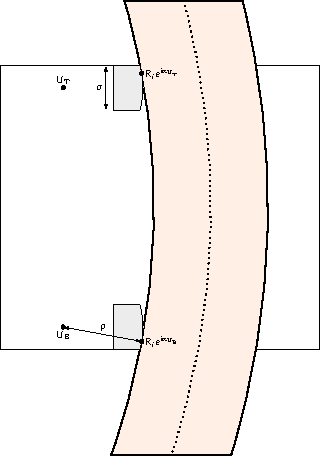
\includegraphics{RfCPN_p05_pictures/mouldUkeita.pdf}}%
\vfill~
\captionof{figure}[\ReceiverPlate がある場合]{%
 \ReceiverPlate がある場合\newline
 $\rho$, $\sigma$は\ReceiverPlateRadius および\ReceiverPlateWidth を示し、U$_\mathrm T$, U$_\mathrm B$はそれぞれの\ReceiverPlateCenter を示す。
 \ReceiverPlate があると\index{ワーク}ワークとの\index{せってん(ワークとうけいた)@接点(ワークと受板)}接点U$_\mathrm B$の位置も変化する。
 なお\ReceiverPlate は、トップ側とボトム側で同じものであり、その片面は\Jig の片面と揃える形で装着されるものとする。
 }%\label{fig:mouldwithukeita}
\end{Figbox}%
\end{figure}%
%%%%%%%%%%%%%%%%%%%%%%%%%%%%%%%%%%%%%%%%%%%%%%%%%%%%%%%%%%
%%%%%%%%%%%%%%%%%%%%%%%%%%%%%%%%%%%%%%%%%%%%%%%%%%%%%%%%%%
%%%%%%%%%%%%%%%%%%%%%%%%%%%%%%%%%%%%%%%%%%%%%%%%%%%%%%%%%%
\ReceiverPlateCenter を改めてU$_\mathrm B$とし、また\index{げんてんO@原点O}原点Oに対する\index{へんかく(\yomiReceiverPlate)@偏角(\nameReceiverPlate)}偏角を改めて$-\alpha_{\mathrm U_\mathrm B}$とすると、これはU$_\mathrm B$($R_\mathrm i-\rho$, $-\alpha_{\mathrm U_\mathrm B}$)と表すことができる。
ただし、\pageeqref{eq:constraintUpoint2}は以下のようになる。
\begin{align*}
  \sin\alpha_{\mathrm U_\mathrm B} = \frac{\bar l}{R_\mathrm i-\rho}\quad, \quad
  \tan\psi = \frac{\delta_\mathrm s}{2\bar l} \quad
  \ab(~\bar l \equiv l-\frac\sigma2~).
\end{align*}
これを原点Oを中心に$\Omega$だけ回転し、さらに点U$_\mathrm B$($R_\mathrm i-\rho$, $-\alpha_{\mathrm U_\mathrm B}$)を中心に点T$_\mathrm i$($R_\mathrm i$, $\alpha_{\mathrm T_\mathrm i}$)を$-\theta$だけ回転すると、
%% label{eq:afterftUfinite}
\begin{align}
  \notag
  & e^{-i\theta}\!
    \ab\{R_\mathrm ie^{i(\alpha_{\mathrm T_\mathrm i}+\Omega)}
           -R_\mathrm i'e^{-i\alpha_{\mathrm U_\mathrm B}}\}
    +R_\mathrm i'e^{-i\alpha_{\mathrm U_\mathrm B}}\\
  & = R_\mathrm ie^{i(\alpha_{\mathrm T_\mathrm i}+\Omega-\theta)}
      -R_\mathrm i'\!
       \ab\{e^{-i(\alpha_{\mathrm U_\mathrm B}+\theta)}-e^{-i\alpha_{\mathrm U_\mathrm B}}\}\qquad
    \big(R_\mathrm i' \equiv R_\mathrm i-\rho\big)
    \label{eq:afterftUfinite}
\end{align}
に移動する。
同様に点T$_\mathrm o$($R_\mathrm o$, $\alpha_{\mathrm T_\mathrm o}$)は
\begin{align*}
  R_\mathrm oe^{i(\alpha_{\mathrm T_\mathrm o}+\Omega-\theta)}
  -R_\mathrm i'\!
   \ab\{e^{-i(\alpha_{\mathrm U_\mathrm B} + \theta)} - e^{-i\alpha_{\mathrm U_\mathrm B}}\}
\end{align*}
に移動する。
したがって、これらの差
\begin{align*}
  e^{i(\Omega-\theta)}
  \ab(R_\mathrm oe^{i\alpha_{\mathrm T_\mathrm o}} - R_\mathrm ie^{i\alpha_{\mathrm T_\mathrm i}})
\end{align*}
の虚部が0であればよい。
つまり、\pageeqref{eq:constraintUpoint1}より、\ReceiverPlate がある場合も$\Omega = \theta$である。


%%%%%%%%%%%%%%%%%%%%%%%%%%%%%%%%%%%%%%%%%%%%%%%%%%%%%%%%%%
%% subsection 20.2.1 %%%%%%%%%%%%%%%%%%%%%%%%%%%%%%%%%%%%%
%%%%%%%%%%%%%%%%%%%%%%%%%%%%%%%%%%%%%%%%%%%%%%%%%%%%%%%%%%
\subsection{\ReceiverPlateContactPoint}
\ReceiverPlate と\index{ワーク}ワークとの(トップ側の)接点は、$R_\mathrm ie^{i\alpha_{\mathrm U_\mathrm B}}$で与えられる。
このとき厚さ$\delta_\mathrm s$の\Spacer を取付けると、U$_\mathrm B$を中心に回転するが、それに伴い\ReceiverPlateContactPoint の位置も変化する。

%%%%%%%%%%%%%%%%%%%%%%%%%%%%%%%%%%%%%%%%%%%%%%%%%%%%%%%%%%
%% subsubsection 19.2.1.1 %%%%%%%%%%%%%%%%%%%%%%%%%%%%%%%%
%%%%%%%%%%%%%%%%%%%%%%%%%%%%%%%%%%%%%%%%%%%%%%%%%%%%%%%%%%
\subsubsection{\expandafterindex{かいてんごの\yomiCurvatureCenter@回転後の\nameCurvatureCenter}回転後のワークの\nameCurvatureCenter}
%%%%%%%%%%%%%%%%%%%%%%%%%
厚さ$\delta_\mathrm s$の\Spacer を挟むと、\TopSideReceiverPlateCenter U$_\mathrm B$は実軸方向に$\delta_\mathrm s$だけ移動するので、
\begin{align*}
  R_\mathrm i'e^{i\alpha_{\mathrm U_\mathrm B}}
  \quad\longrightarrow\quad
  \delta_\mathrm s+R_\mathrm i'e^{i\alpha_{\mathrm U_\mathrm B}}\ .
\end{align*}
よって、それぞれの\ReceiverPlateCenter U$_\mathrm B$, U$_\mathrm T$を結んだ線分U$_\mathrm B$U$_\mathrm T$は、U$_\mathrm B$を中心に$-\psi$だけ傾いた線分U$_\mathrm B'$U$_\mathrm T'$となる
%% footnote %%%%%%%%%%%%%%%%%%%%%
\footnote{%
U$_\mathrm B'$U$_\mathrm T'$の長さは$\bar l\sec\psi$であり、U$_\mathrm B$U$_\mathrm T$の長さ$\bar l$より長くなることに注意。}。
%%%%%%%%%%%%%%%%%%%%%%%%%%%%%%%%%
\expandafterindex{かいてんごの\yomiCurvatureCenter@回転後の\nameCurvatureCenter}回転後の\nameCurvatureCenter は、この線分の垂直二等分線上にあり、またそれぞれの\ReceiverPlateCenter から$R_\mathrm i'$の距離の位置にある。
つまり、この傾いた線分U$_\mathrm B'$U$_\mathrm T'$の中点から、角度$\pi-\psi$, 大きさ$\sqrt{R_\mathrm i'^2-\frac{\delta_\mathrm s^2+(2\bar l)^2}4}$の位置に移動する。
したがって、回転後における\CurvatureCenter O$'$は、
%% label{eq:afterOrgin}
\begin{align}
  \notag
  & \frac{\delta_\mathrm s}2+\sqrt{R_\mathrm i'^2-\bar l^2}
    +\sqrt{R_\mathrm i'^2-\frac{\delta_\mathrm s^2+(2\bar l)^2}4}e^{i(\pi-\psi)}\\
  & = \frac{\delta_\mathrm s}2+\sqrt{R_\mathrm i'^2-\bar l^2}-\sqrt{R_\mathrm i'^2-\frac{\delta_\mathrm s^2+(2\bar l)^2}4}\cos\psi
      +i\sqrt{R_\mathrm i'^2-\frac{\delta_\mathrm s^2+(2\bar l)^2}4}\sin\psi\ .
    \label{eq:afterOrgin}
\end{align}

%\clearpage
%%%%%%%%%%%%%%%%%%%%%%%%%%%%%%%%%%%%%%%%%%%%%%%%%%%%%%%%%%
%% subsubsection 19.2.1.2 %%%%%%%%%%%%%%%%%%%%%%%%%%%%%%%%
%%%%%%%%%%%%%%%%%%%%%%%%%%%%%%%%%%%%%%%%%%%%%%%%%%%%%%%%%%
\subsubsection{\AfterRotatePlateContactPoint(トップ側)}
\AfterRotateReceiverPlateCenter U$_\mathrm T'$と\expandafterindex{かいてんごの\yomiCurvatureCenter@回転後の\nameCurvatureCenter}\nameCurvatureCenter O$'$との差をとると、
\begin{align*}
  \frac{\delta_\mathrm s}2+\sqrt{R_\mathrm i'^2-\frac{\delta_\mathrm s^2+(2\bar l)^2}4}\cos\psi
  +i\ab\{\bar l-\sqrt{R_\mathrm i'^2-\frac{\delta_\mathrm s^2+(2\bar l)^2}4}\sin\psi\}
  = R_\mathrm i'e^{i\alpha'_{\mathrm U_\mathrm T}}\ .
\end{align*}
ここで、
\begin{align*}
  \tan\alpha'_{\mathrm U_\mathrm T}
  = \frac{\displaystyle\bar l-\sqrt{R_\mathrm i'^2-\frac{\delta_\mathrm s^2+(2\bar l)^2}4}\sin\psi}
         {\displaystyle\frac{\delta_\mathrm s}2+\sqrt{R_\mathrm i'^2-\frac{\delta_\mathrm s^2+(2\bar l)^2}4}\cos\psi}\ .
\end{align*}
%%%%%%%%%%%%%%%%%%%%%%%%%%%%%%%%%%%%%%%%%%%%%%%%%%%%%%%%%%
%% hosoku %%%%%%%%%%%%%%%%%%%%%%%%%%%%%%%%%%%%%%%%%%%%%%%%
%%%%%%%%%%%%%%%%%%%%%%%%%%%%%%%%%%%%%%%%%%%%%%%%%%%%%%%%%%
\begin{hosoku}
これの大きさは、$\delta_\mathrm s\cos\psi-2\bar l\sin\psi = 0$より、
\begin{align*}
  \ab\{\frac{\delta_\mathrm s}2+\sqrt{R_\mathrm i'^2-\frac{\delta_\mathrm s^2+(2\bar l)^2}4}\cos\psi\}^2
  +\ab\{\bar l-\sqrt{R_\mathrm i'^2-\frac{\delta_\mathrm s^2+(2\bar l)^2}4}\sin\psi\}^2
  = R_\mathrm i'^2\ .
\end{align*}
\end{hosoku}
%%%%%%%%%%%%%%%%%%%%%%%%%%%%%%%%%%%%%%%%%%%%%%%%%%%%%%%%%%
%%%%%%%%%%%%%%%%%%%%%%%%%%%%%%%%%%%%%%%%%%%%%%%%%%%%%%%%%%
%%%%%%%%%%%%%%%%%%%%%%%%%%%%%%%%%%%%%%%%%%%%%%%%%%%%%%%%%%
よって、\AfterRotatePlateContactPoint は以下で与えられる。
\begin{align*}
  &  R_\mathrm ie^{i\alpha'_{\mathrm U_\mathrm T}}
     +\frac{\delta_\mathrm s}2+\sqrt{R_\mathrm i'^2-\bar l^2}-\sqrt{R_\mathrm i'^2-\frac{\delta_\mathrm s^2+(2\bar l)^2}4}\cos\psi
     +i\sqrt{R_\mathrm i'^2-\frac{\delta_\mathrm s^2+(2\bar l)^2}4}\sin\psi\\
  &= \delta_\mathrm s+R_\mathrm i'e^{i\alpha_{\mathrm U_\mathrm B}}+\rho e^{i\alpha'_{\mathrm U_\mathrm T}}\ .
\end{align*}

%\clearpage
%%%%%%%%%%%%%%%%%%%%%%%%%%%%%%%%%%%%%%%%%%%%%%%%%%%%%%%%%%
%% subsubsection 1.2.1.3 %%%%%%%%%%%%%%%%%%%%%%%%%%%%%%%%%
%%%%%%%%%%%%%%%%%%%%%%%%%%%%%%%%%%%%%%%%%%%%%%%%%%%%%%%%%%
\subsubsection{\AfterRotatePlateContactPoint(ボトム側)}
\AfterRotateBottomSideReceiverPlateCenter U$_\mathrm B$と\CurvatureCenter O$'$との差をとると、
\begin{align*}
  -\frac{\delta_\mathrm s}2+\sqrt{R_\mathrm i'^2-\frac{\delta_\mathrm s^2+(2\bar l)^2}4}\cos\psi
  -i\ab\{\bar l+\sqrt{R_\mathrm i'^2-\frac{\delta_\mathrm s^2+(2\bar l)^2}4}\sin\psi\}
  = R_\mathrm i'e^{-i\alpha'_{\mathrm U_\mathrm B}}
\end{align*}
ここで、
\begin{align*}
  \tan\alpha'_{\mathrm U_\mathrm B}
  = \frac{\displaystyle\bar l+\sqrt{R_\mathrm i'^2-\frac{\delta_\mathrm s^2+(2\bar l)^2}4}\sin\psi}
         {\displaystyle-\frac{\delta_\mathrm s}2+\sqrt{R_\mathrm i'^2-\frac{\delta_\mathrm s^2+(2\bar l)^2}4}\cos\psi}
\end{align*}
よって、\AfterRotatePlateContactPoint は以下で与えられる。
%% label{eq:afterUBcontact}
\begin{align}
  \notag
  &  R_\mathrm ie^{-i\alpha'_{\mathrm U_\mathrm B}}
     +\frac{\delta_\mathrm s}2+\sqrt{R_\mathrm i'^2-\bar l^2}-\sqrt{R_\mathrm i'^2-\frac{\delta_\mathrm s^2+(2\bar l)^2}4}\cos\psi
     +i\sqrt{R_\mathrm i'^2-\frac{\delta_\mathrm s^2+(2\bar l)^2}4}\sin\psi\\
  &= R_\mathrm i'e^{-i\alpha_{\mathrm U_\mathrm B}}+\rho e^{-i\alpha'_{\mathrm U_\mathrm B}}
   \label{eq:afterUBcontact}
\end{align}
%%%%%%%%%%%%%%%%%%%%%%%%%%%%%%%%%%%%%%%%%%%%%%%%%%%%%%%%%%
%% hosoku %%%%%%%%%%%%%%%%%%%%%%%%%%%%%%%%%%%%%%%%%%%%%%%%
%%%%%%%%%%%%%%%%%%%%%%%%%%%%%%%%%%%%%%%%%%%%%%%%%%%%%%%%%%
\begin{hosoku}
辺の長さが$R_i'$, $R_i'$, $2\bar l$の二等辺三角形$\triangle$OU$_\mathrm B$U$_\mathrm T$の部分が、傾き後には辺の長さ$R_i'$, $R_i'$, $\sqrt{\delta_\mathrm s^2+(2\bar l)^2}$の二等辺三角形$\triangle$O$'$U$_\mathrm B'$U$_\mathrm T'$となる。
実際、$\cos2a = 1-2\sin^2\!a$より、
\begin{align*}
  \sin^2\frac{\alpha'_{\mathrm U_\mathrm T}+\alpha'_{\mathrm U_\mathrm B}}2
  = \frac{\delta_\mathrm s^2+(2\bar l)^2}{4R_\mathrm i'^2}\ .
\end{align*}
\end{hosoku}
%%%%%%%%%%%%%%%%%%%%%%%%%%%%%%%%%%%%%%%%%%%%%%%%%%%%%%%%%%
%%%%%%%%%%%%%%%%%%%%%%%%%%%%%%%%%%%%%%%%%%%%%%%%%%%%%%%%%%
%%%%%%%%%%%%%%%%%%%%%%%%%%%%%%%%%%%%%%%%%%%%%%%%%%%%%%%%%%


%%%%%%%%%%%%%%%%%%%%%%%%%%%%%%%%%%%%%%%%%%%%%%%%%%%%%%%%%%
%% subsection 1.2.2 %%%%%%%%%%%%%%%%%%%%%%%%%%%%%%%%%%%%%%
%%%%%%%%%%%%%%%%%%%%%%%%%%%%%%%%%%%%%%%%%%%%%%%%%%%%%%%%%%
\subsection{\Spacer による\index{かたむきかく(スペーサ)@傾き角(スペーサ)}ワークの傾き角}
厚さ$\delta_\mathrm s$の\Spacer を挿入すると、\CurvatureCenter Oは、U$_\mathrm B$を中心に$-\big(\alpha'_{\mathrm U_\mathrm B}\!-\alpha_{\mathrm U_\mathrm B}\big)$だけ回転する。
実際、
\begin{align*}
  -R_\mathrm i'e^{-i\alpha'_{\mathrm U_\mathrm B}}+R_\mathrm i'e^{-i\alpha_{\mathrm U_\mathrm B}}
  &= R_\mathrm i'(\cos\alpha_{\mathrm U_\mathrm B}-\cos\alpha'_{\mathrm U_\mathrm B})
     +iR_\mathrm i'(\sin\alpha'_{\mathrm U_\mathrm B}-\sin\alpha_{\mathrm U_\mathrm B})
\end{align*}
であり、これは\expandafterindex{かいてんごの\yomiCurvatureCenter@回転後の\nameCurvatureCenter}回転後の\nameCurvatureCenter\pageeqref{eq:afterOrgin}に一致する。
つまり、$\alpha'_{\mathrm U_\mathrm B}\!-\alpha_{\mathrm U_\mathrm B}$が$\theta$に相当する。
%%%%%%%%%%%%%%%%%%%%%%%%%%%%%%%%%%%%%%%%%%%%%%%%%%%%%%%%%%
%% hosoku %%%%%%%%%%%%%%%%%%%%%%%%%%%%%%%%%%%%%%%%%%%%%%%%
%%%%%%%%%%%%%%%%%%%%%%%%%%%%%%%%%%%%%%%%%%%%%%%%%%%%%%%%%%
\begin{hosoku}
\TopSideReceiverPlateContactPoint U$_\mathrm T'$と\BottomSideReceiverPlateContactPoint U$_\mathrm B'$の差をとると、
\begin{align*}
  R_\mathrm i\ab(e^{i\alpha_{\mathrm U_\mathrm T}'}-e^{-i\alpha'_{\mathrm U_\mathrm B}})
  &= \frac{R_\mathrm i'+\rho}{R_\mathrm i'}\ab\{\delta_\mathrm s+i(2\bar l)\}
   = \frac{R_\mathrm i}{R_\mathrm i'}\sqrt{\delta_\mathrm s^2+(2\bar l)^2}e^{i(\nicefrac\pi2-\psi)}\ .
\end{align*}
したがって、厚さ$\delta_\mathrm s$の\Spacer を挿入すると、両接点を通る直線は$-\psi$だけ傾くことがわかる。
また、その長さは\ReceiverPlateCenter 間U$_\mathrm T'$U$_\mathrm B'$の距離$\sqrt{\delta_\mathrm s^2+(2\bar l)^2}$の$\nicefrac{R_i}{R_i'}$倍になっていることも確かめられる。
\end{hosoku}
%%%%%%%%%%%%%%%%%%%%%%%%%%%%%%%%%%%%%%%%%%%%%%%%%%%%%%%%%%
%%%%%%%%%%%%%%%%%%%%%%%%%%%%%%%%%%%%%%%%%%%%%%%%%%%%%%%%%%
%%%%%%%%%%%%%%%%%%%%%%%%%%%%%%%%%%%%%%%%%%%%%%%%%%%%%%%%%%


%%%%%%%%%%%%%%%%%%%%%%%%%%%%%%%%%%%%%%%%%%%%%%%%%%%%%%%%%%
%% subsection 1.2.3 %%%%%%%%%%%%%%%%%%%%%%%%%%%%%%%%%%%%%%
%%%%%%%%%%%%%%%%%%%%%%%%%%%%%%%%%%%%%%%%%%%%%%%%%%%%%%%%%%
\subsection{\Spacer による\ReAlocation}

%%%%%%%%%%%%%%%%%%%%%%%%%%%%%%%%%%%%%%%%%%%%%%%%%%%%%%%%%%
%% subsubsection 1.2.3.1 %%%%%%%%%%%%%%%%%%%%%%%%%%%%%%%%%
%%%%%%%%%%%%%%%%%%%%%%%%%%%%%%%%%%%%%%%%%%%%%%%%%%%%%%%%%%
\subsubsection{\ReAlocationLength}
\Spacer を入れた後の\TopAlocationLength(\textbf{\TopReAlocationLength})$f'_\mathrm T$は、\pageeqref{eq:afterftUfinite}の虚部を見ればよい。
回転角は$-(\alpha'_{\mathrm U_\mathrm B}-\alpha_{\mathrm U_\mathrm B})$なので、
\begin{align*}
  f'_\mathrm T
  = R_\mathrm i\sin\alpha_{\mathrm T_\mathrm i}
    +R_\mathrm i'\ab(\sin\alpha'_{\mathrm U_\mathrm B}-\sin\alpha_{\mathrm U_\mathrm B})
  &= f_\mathrm T+\sqrt{R_\mathrm i'^2-\frac{\delta_\mathrm s^2+(2\bar l)^2}4}\sin\psi\\
  &= f_\mathrm T+\sqrt{R_\mathrm i'^2-\frac{\delta_\mathrm s^2+(2\bar l)^2}4}\frac{\delta_\mathrm s}{\sqrt{\delta_\mathrm s^2+(2\bar l)^2}}\ .
\end{align*}

%%%%%%%%%%%%%%%%%%%%%%%%%%%%%%%%%%%%%%%%%%%%%%%%%%%%%%%%%%
%% subsubsection 1.2.3.2 %%%%%%%%%%%%%%%%%%%%%%%%%%%%%%%%%
%%%%%%%%%%%%%%%%%%%%%%%%%%%%%%%%%%%%%%%%%%%%%%%%%%%%%%%%%%
\subsubsection{\index{ワーク}ワークの移動距離}
\pageeqref{eq:afterftUfinite}の実部は、
\begin{align*}
  & R_\mathrm i\cos\alpha_{\mathrm T_\mathrm i}
    -R_\mathrm i'(\cos\alpha'_{\mathrm U_\mathrm B}-\cos\alpha_{\mathrm U_\mathrm B})\\
  & = \sqrt{R_\mathrm i^2-f_\mathrm T^2}+\frac{\delta_\mathrm s}2+\sqrt{R_\mathrm i'^2-\bar l^2}
      -\sqrt{R_\mathrm i'^2-\frac{\delta_\mathrm s^2+(2\bar l)^2}4}\cos\psi
\end{align*}
となる。
よって、\Spacer を挿入することにより、\index{ワーク}ワークは水平・鉛直方向にそれぞれ、
\begin{alignat}{2}
%% label{eq:spacerMoveHdistance}
  \label{eq:spacerMoveHdistance}
  \text{水平方向:}\quad
  & \frac{\delta_\mathrm s}2+\sqrt{R_\mathrm i'^2-\bar l^2}-\sqrt{R_\mathrm i'^2-\frac{\delta_\mathrm s^2+(2\bar l)^2}4}\frac{2\bar l}{\sqrt{\delta_\mathrm s^2+(2\bar l)^2}}\\
  \notag
  \text{鉛直方向:}\quad
  & \sqrt{R_\mathrm i'^2-\frac{\delta_\mathrm s^2+(2\bar l)^2}4}\frac{\delta_\mathrm s}{\sqrt{\delta_\mathrm s^2+(2\bar l)^2}}
\end{alignat}
だけ移動することがわかる。


%\clearpage
%%%%%%%%%%%%%%%%%%%%%%%%%%%%%%%%%%%%%%%%%%%%%%%%%%%%%%%%%%
%% subsection 1.2.4 %%%%%%%%%%%%%%%%%%%%%%%%%%%%%%%%%%%%%%
%%%%%%%%%%%%%%%%%%%%%%%%%%%%%%%%%%%%%%%%%%%%%%%%%%%%%%%%%%
\subsection{\ReAlocationLength が均等になる\SpacerThickness}
トップ側とボトム側の\index{きんとうふりわけ@均等振分}\AlocationLength が同じになるとき、$\delta_\mathrm s$は
\begin{align}
  \label{eq:condtionequalalocationSpacer}
  \sqrt{R_\mathrm i'^2-\frac{\delta_\mathrm s^2+(2\bar l)^2}4}\frac{\delta_\mathrm s}{\sqrt{\delta_\mathrm s^2+(2\bar l)^2}} = f_d \qquad
  \ab(f_d \equiv \frac{f_\mathrm B-f_\mathrm T}2)\ .
\end{align}
を満たす。
これより、
\begin{align*}
  \delta_\mathrm s^2
  &= \ab(\sqrt{R_\mathrm i'^2-(\bar l-f_d)^2}-\sqrt{R_\mathrm i'^2-(\bar l+f_d)^2}\,)^2.
\end{align*}
なお、これはワークが水平・鉛直方向にそれぞれ、
\begin{align*}
  \text{水平方向:}~\frac{\delta_\mathrm s}2+\sqrt{R_\mathrm i^2-\bar l^2}-\frac{2\bar l}{\delta_\mathrm s}f_d\quad(\delta_\mathrm s>0)\ , \qquad
  \text{鉛直方向:}~\frac{f_\mathrm B-f_\mathrm T}2
\end{align*}
だけ移動することを意味する。
%%%%%%%%%%%%%%%%%%%%%%%%%%%%%%%%%%%%%%%%%%%%%%%%%%%%%%%%%%
%% hosoku %%%%%%%%%%%%%%%%%%%%%%%%%%%%%%%%%%%%%%%%%%%%%%%%
%%%%%%%%%%%%%%%%%%%%%%%%%%%%%%%%%%%%%%%%%%%%%%%%%%%%%%%%%%
\begin{hosoku}
\pageeqref{eq:condtionequalalocationSpacer}の両辺を2乗して$-4$倍すると、
\begin{align*}
  \delta_\mathrm s^2\ab\{\delta_\mathrm s^2+(2\bar l)^2-4R_\mathrm i'^2\}+4f_d^2\ab\{\delta_\mathrm s^2+(2\bar l)^2\}
  & = \delta_\mathrm s^4-2\ab\{2R_\mathrm i'^2-2\bar l^2-2f_d^2\}\delta_\mathrm s^2+4f_d^2(2\bar l)^2
    = 0\ .
\end{align*}
したがって、$f_\mathrm T = f_\mathrm B$ ($f_d = 0$)のとき$\delta_\mathrm s = 0$であることを考慮して、
\begin{align*}
  \delta_\mathrm s^2
  &= 2\ab\{
       R_\mathrm i'^2-\bar l^2-f_d^2-\sqrt{\ab(R_\mathrm i'^2-\bar l^2-f_d^2)^2-4f_d^2\bar l^2}\,
     \}\\
  &= \ab(\sqrt{R_\mathrm i'^2-(\bar l-f_d)^2}-\sqrt{R_\mathrm i'^2-(\bar l+f_d)^2}\,)^2.
\end{align*}
\end{hosoku}
%%%%%%%%%%%%%%%%%%%%%%%%%%%%%%%%%%%%%%%%%%%%%%%%%%%%%%%%%%
%%%%%%%%%%%%%%%%%%%%%%%%%%%%%%%%%%%%%%%%%%%%%%%%%%%%%%%%%%
%%%%%%%%%%%%%%%%%%%%%%%%%%%%%%%%%%%%%%%%%%%%%%%%%%%%%%%%%%
%%%%%%%%%%%%%%%%%%%%%%%%%%%%%%%%%%%%%%%%%%%%%%%%%%%%%%%%%%
%% hosoku %%%%%%%%%%%%%%%%%%%%%%%%%%%%%%%%%%%%%%%%%%%%%%%%
%%%%%%%%%%%%%%%%%%%%%%%%%%%%%%%%%%%%%%%%%%%%%%%%%%%%%%%%%%
\begin{hosoku}
改めてまとめると、厚さ$\delta_\mathrm s$の\Spacer を(トップ側に)挿入した後の\TopAlocationLength$f_\mathrm T'$は、
\begin{align*}
  f_\mathrm T'
  = f_\mathrm T+\sqrt{R_\mathrm i'^2-\frac{\delta_\mathrm s^2+(2\bar l)^2}4}\frac{\delta_\mathrm s}{\sqrt{\delta_\mathrm s^2+(2\bar l)^2}}\ .
\end{align*}
トップ側とボトム側の\index{きんとうふりわけ@均等振分}\AlocationLength が均等になるときの\SpacerThickness$\delta_\mathrm s'$は、
\begin{align*}
  \delta_\mathrm s' = \sqrt{R_\mathrm i'^2-(\bar l-f_d)^2}-\sqrt{R_\mathrm i'^2-(\bar l+f_d)^2}\ .
\end{align*}
ここで、
\begin{align*}
  R_\mathrm i' = R_\mathrm c-\frac{W_x}2-\rho\ ,\quad
  \bar l = l-\frac\sigma2\ ,\quad
  f_d = \frac{f_\mathrm B-f_\mathrm T}2\ .
\end{align*}
\end{hosoku}
%%%%%%%%%%%%%%%%%%%%%%%%%%%%%%%%%%%%%%%%%%%%%%%%%%%%%%%%%%
%%%%%%%%%%%%%%%%%%%%%%%%%%%%%%%%%%%%%%%%%%%%%%%%%%%%%%%%%%
%%%%%%%%%%%%%%%%%%%%%%%%%%%%%%%%%%%%%%%%%%%%%%%%%%%%%%%%%%



\clearpage
%%%%%%%%%%%%%%%%%%%%%%%%%%%%%%%%%%%%%%%%%%%%%%%%%%%%%%%%%%
%% section 21.3 %%%%%%%%%%%%%%%%%%%%%%%%%%%%%%%%%%%%%%%%%%
%%%%%%%%%%%%%%%%%%%%%%%%%%%%%%%%%%%%%%%%%%%%%%%%%%%%%%%%%%
\modHeadsection{\Table の回転による\AlocationLength の調節}
これまで\TopAlocationLength・\BottomAlocationLength の差を小さくするために\Spacer を用いる手法を考えてきた。
\Spacer を取付けることは、本質的にはボトム側の\ReceiverPlate の点U$_\mathrm B$を中心に回転しているということである。
このとき回転の中心はU$_\mathrm B$である必要はなく、他の点でも問題ない。
したがって、\Spacer を用いて回転をしなくても、\Table そのものを回転するという手法が考えられる。
これは回転の中心が、\ReceiverPlateCenter U$_\mathrm B$から\textbf{\TableCenter}Pに変わることに相当する。

\ReceiverPlateCenter U$_\mathrm B$と、\TableCenter Pとの実軸方向の距離を$\Delta_x$とすると、\TableCenter Pの$X$座標$\Delta_x'$は次で与えられる。
%% label{eq:tableCenter}
\begin{align}
  \label{eq:tableCenter}
  \Delta_x'
  = \Delta_x+R_\mathrm i'\cos\alpha_{\mathrm U_\mathrm B} = \Delta_x+\sqrt{R_\mathrm i'^2-\bar l^2}\ .
\end{align}
\index{トップがわのCがわそとたんてん@トップ側のC側外端点}トップ側のC側外端点T$_\mathrm i$($R_\mathrm i$, $\alpha_{\mathrm T_\mathrm i}$)を、原点Oを中心に$\Omega$だけ回転し、さらに点P\,($\Delta_x'$, $0$)を中心に$-\theta$だけ回転すると、
\begin{align}
  \label{eq:afterfttable}
  e^{-i\theta}\ab\{R_\mathrm i^{i(\alpha_{\mathrm T_\mathrm i}+\Omega)}-\Delta_x'\}+\Delta_x'
  = R_\mathrm ie^{i(\alpha_{\mathrm T_\mathrm i}+\Omega-\theta)}+\Delta_x'\ab(1-e^{-i\theta})
\end{align}
に移動する。
同様に、\index{トップがわのAがわそとたんてん@トップ側のA側外端点}トップ側のA側外端点T$_\mathrm o$($R_\mathrm o$, $\alpha_{\mathrm T_\mathrm o}$)は、
\begin{align*}
  e^{-i\theta}\!\ab\{R_\mathrm o^{i(\alpha_{\mathrm T_\mathrm o}+\Omega)}-\Delta_x'\}+\Delta_x'
  = R_\mathrm ie^{i(\alpha_{\mathrm T_\mathrm o}+\Omega-\theta)}+\Delta_x'\!\ab(1-e^{-i\theta})
\end{align*}
に移動する。
したがって、これらの差
\begin{align*}
  e^{i(\Omega-\theta)}
  \ab(R_\mathrm oe^{i\alpha_{\mathrm T_\mathrm o}}-R_\mathrm ie^{i\alpha_{\mathrm T_\mathrm i}})
\end{align*}
の虚部が$0$であればよい。
よって\pageeqref{eq:constraintUpoint1}より、この場合も$\Omega = \theta$となる。


%%%%%%%%%%%%%%%%%%%%%%%%%%%%%%%%%%%%%%%%%%%%%%%%%%%%%%%%%%
%% subsection 21.3.1 %%%%%%%%%%%%%%%%%%%%%%%%%%%%%%%%%%%%%
%%%%%%%%%%%%%%%%%%%%%%%%%%%%%%%%%%%%%%%%%%%%%%%%%%%%%%%%%%
\subsection{回転後の\CurvatureCenter および\ReceiverPlateContactPoint}

%%%%%%%%%%%%%%%%%%%%%%%%%%%%%%%%%%%%%%%%%%%%%%%%%%%%%%%%%%
%% subsubsection 21.3.1.1 %%%%%%%%%%%%%%%%%%%%%%%%%%%%%%%%
%%%%%%%%%%%%%%%%%%%%%%%%%%%%%%%%%%%%%%%%%%%%%%%%%%%%%%%%%%
\subsubsection{回転後の\index{ワーク}ワークの\CurvatureCenter}
\expandafterindex{かいてんごの\yomiCurvatureCenter@回転後の\nameCurvatureCenter}回転後の\nameCurvatureCenter O$'$は、点Pを中心に$-\theta$だけ回転するので、
\begin{align*}
  \Delta_x'\!\ab(1-e^{-i\theta}) = \Delta_x'(1-\cos\theta)+i\Delta_x'\sin\theta\ .
\end{align*}

%%%%%%%%%%%%%%%%%%%%%%%%%%%%%%%%%%%%%%%%%%%%%%%%%%%%%%%%%%
%% subsubsection 21.3.1.2 %%%%%%%%%%%%%%%%%%%%%%%%%%%%%%%%
%%%%%%%%%%%%%%%%%%%%%%%%%%%%%%%%%%%%%%%%%%%%%%%%%%%%%%%%%%
\subsubsection{\AfterRotatePlateContactPoint}
傾き後における\TopSideReceiverPlateContactPoint は、点Pを中心に$-\theta$だけ回転するので、
\begin{align*}
  &  e^{-i\theta}\ab(R_\mathrm ie^{i\alpha_{\mathrm U_\mathrm B}}-\Delta_x')+\Delta_x'\\
  &= R_\mathrm ie^{i(\alpha_{\mathrm U_\mathrm B}-\theta)}+\Delta_x'\!\ab(1-e^{-i\theta})\\
  &= R_\mathrm i\cos(\alpha_{\mathrm U_\mathrm B}-\theta)+\Delta_x'(1-\cos\theta)
     +i\ab\{R_\mathrm i\sin(\alpha_{\mathrm U_\mathrm B}-\theta)+i\Delta_x'\sin\theta\}\ .
\end{align*}
同様に、傾き後における\BottomSideReceiverPlateContactPoint は、
\begin{align*}
  &  e^{-i\theta}\ab(R_\mathrm ie^{-i\alpha_{\mathrm U_\mathrm B}}-\Delta_x')+\Delta_x'\\
  &= R_\mathrm ie^{-i(\alpha_{\mathrm U_\mathrm B}+\theta)}+\Delta_x'\!\ab(1-e^{-i\theta})\\
  &= R_\mathrm i\cos(\alpha_{\mathrm U_\mathrm B}+\theta)+\Delta_x'(1-\cos\theta)
     -i\ab\{R_\mathrm i\sin(\alpha_{\mathrm U_\mathrm B}+\theta)-i\Delta_x'\sin\theta\}\ .
\end{align*}
%%%%%%%%%%%%%%%%%%%%%%%%%%%%%%%%%%%%%%%%%%%%%%%%%%%%%%%%%%
%% hosoku %%%%%%%%%%%%%%%%%%%%%%%%%%%%%%%%%%%%%%%%%%%%%%%%
%%%%%%%%%%%%%%%%%%%%%%%%%%%%%%%%%%%%%%%%%%%%%%%%%%%%%%%%%%
\begin{hosoku}
両接点との差をとると、
\begin{align*}
  2R_\mathrm i\sin\alpha_{\mathrm U_\mathrm B}\sin\theta+2iR_\mathrm i\sin\alpha_{\mathrm U_\mathrm B}\cos\theta
  = \frac{R_\mathrm i}{R_\mathrm i'}(2\bar l)e^{i(\pi-\theta)}
\end{align*}
となり、\ReceiverPlate の両中心間(長さ$2\bar l$)を結んだ線分を$\nicefrac{R_\mathrm i}{R_\mathrm i'}$倍し、虚軸から$-\theta$だけ傾けたものになっていることがわかる。
\end{hosoku}
%%%%%%%%%%%%%%%%%%%%%%%%%%%%%%%%%%%%%%%%%%%%%%%%%%%%%%%%%%
%%%%%%%%%%%%%%%%%%%%%%%%%%%%%%%%%%%%%%%%%%%%%%%%%%%%%%%%%%
%%%%%%%%%%%%%%%%%%%%%%%%%%%%%%%%%%%%%%%%%%%%%%%%%%%%%%%%%%


%%%%%%%%%%%%%%%%%%%%%%%%%%%%%%%%%%%%%%%%%%%%%%%%%%%%%%%%%%
%% subsection 21.3.2 %%%%%%%%%%%%%%%%%%%%%%%%%%%%%%%%%%%%%
%%%%%%%%%%%%%%%%%%%%%%%%%%%%%%%%%%%%%%%%%%%%%%%%%%%%%%%%%%
\subsection{傾き後の\AlocationLength}
傾き後の\TopReAlocationLength$f_\mathrm T'$は、\pageeqref{eq:afterfttable}の虚部を見ればよいので、
\begin{align}
  \label{eq:realocationT}
  f_\mathrm T'
  = f_\mathrm T+\Delta_x'\sin\theta
  = f_\mathrm T+\ab(\Delta_x+\sqrt{R_\mathrm i'-\bar l^2})\sin\theta\ .
\end{align}
同様に、\BottomReAlocationLength$f_\mathrm B'$は、符号に注意して、
\begin{align*}
  f_\mathrm B' = f_\mathrm B-\Delta_x'\sin\theta = (f_\mathrm T+f_\mathrm B)-f_\mathrm T'\ .
\end{align*}
%%%%%%%%%%%%%%%%%%%%%%%%%%%%%%%%%%%%%%%%%%%%%%%%%%%%%%%%%%
%% hosoku %%%%%%%%%%%%%%%%%%%%%%%%%%%%%%%%%%%%%%%%%%%%%%%%
%%%%%%%%%%%%%%%%%%%%%%%%%%%%%%%%%%%%%%%%%%%%%%%%%%%%%%%%%%
\begin{hosoku}
\TableCenter Pによる回転は\AlocationLength に影響しない(\EndFace を水平に戻す)ので、\CurvatureCenter Oによる回転だけが影響する。
よって、\AlocationLength は$\Delta_x'\sin\theta$だけ変化する。
\end{hosoku}
%%%%%%%%%%%%%%%%%%%%%%%%%%%%%%%%%%%%%%%%%%%%%%%%%%%%%%%%%%
%%%%%%%%%%%%%%%%%%%%%%%%%%%%%%%%%%%%%%%%%%%%%%%%%%%%%%%%%%
%%%%%%%%%%%%%%%%%%%%%%%%%%%%%%%%%%%%%%%%%%%%%%%%%%%%%%%%%%
なお、\pageeqref{eq:afterfttable}の実部は、
\begin{align*}
  R_\mathrm i\cos\alpha_{\mathrm T_\mathrm i}+\Delta_x'(1-\cos\theta)
  = \sqrt{R_\mathrm i^2-\bar l^2}+\ab(\Delta_x+\sqrt{R_\mathrm i'-\bar l^2})(1-\cos\theta)\ .
\end{align*}
となるので、実軸の正方向に動くことがわかる。


%%%%%%%%%%%%%%%%%%%%%%%%%%%%%%%%%%%%%%%%%%%%%%%%%%%%%%%%%%
%% subsection 21.3.3 %%%%%%%%%%%%%%%%%%%%%%%%%%%%%%%%%%%%%
%%%%%%%%%%%%%%%%%%%%%%%%%%%%%%%%%%%%%%%%%%%%%%%%%%%%%%%%%%
\subsection{\AlocationLength を指定したときの\AlocationAngle}
\TopAlocationLength が$f_\mathrm T'$となる\AlocationAngle$\theta$は、\pageeqref{eq:realocationT}より、
\begin{align}
  \label{eq:alocationangle}
  \sin\theta = \frac{f_\mathrm T'-f_\mathrm T}{\Delta_x'}
\end{align}
で与えられる。
特に、\TopAlocationLength および\BottomAlocationLength が同じになるとき、$\theta$は
\begin{align*}
  \Delta_x'\sin\theta = f_d \qquad \ab(f_d \equiv \frac{f_\mathrm B-f_\mathrm T}2)
\end{align*}
であればいいので、
\begin{align}
  \label{eq:equalalocationangle}
  \sin\theta = \frac{f_d}{\Delta_x'}
  = \frac{f_\mathrm B-f_\mathrm T}{2\ab(\Delta_x+\sqrt{R_\mathrm i'-\bar l^2})}~.
\end{align}
%%%%%%%%%%%%%%%%%%%%%%%%%%%%%%%%%%%%%%%%%%%%%%%%%%%%%%%%%%
%% hosoku %%%%%%%%%%%%%%%%%%%%%%%%%%%%%%%%%%%%%%%%%%%%%%%%
%%%%%%%%%%%%%%%%%%%%%%%%%%%%%%%%%%%%%%%%%%%%%%%%%%%%%%%%%%
\begin{hosoku}
改めてまとめると、\Table を$-\theta$だけ傾けた後の\TopReAlocationLength$f_\mathrm T'$は、
\begin{align*}
  f_\mathrm T' = f_\mathrm T+\ab(\Delta_x+\sqrt{R_\mathrm i'-\bar l^2})\sin\theta\ .
\end{align*}
トップ側とボトム側の\AlocationLength が均等になるときの\AlocationAngle(\textbf{\EqualAlocationAngle})$\theta'$は、
\begin{align*}
  \sin\theta' = \frac{f_\mathrm B-f_\mathrm T}{2\ab(\Delta_x+\sqrt{R_\mathrm i'-\bar l^2})}\ .
\end{align*}
ここで、
\begin{align*}
  R_\mathrm i' = R_\mathrm c-\frac{W_x}2-\rho\ ,\quad
  \bar l = l-\frac\sigma2\ ,\quad
  f_d = \frac{f_\mathrm B-f_\mathrm T}2\ .
\end{align*}
\end{hosoku}
%%%%%%%%%%%%%%%%%%%%%%%%%%%%%%%%%%%%%%%%%%%%%%%%%%%%%%%%%%
%%%%%%%%%%%%%%%%%%%%%%%%%%%%%%%%%%%%%%%%%%%%%%%%%%%%%%%%%%
%%%%%%%%%%%%%%%%%%%%%%%%%%%%%%%%%%%%%%%%%%%%%%%%%%%%%%%%%%



%\clearpage
%%%%%%%%%%%%%%%%%%%%%%%%%%%%%%%%%%%%%%%%%%%%%%%%%%%%%%%%%%
%% section 21.3 %%%%%%%%%%%%%%%%%%%%%%%%%%%%%%%%%%%%%%%%%%
%%%%%%%%%%%%%%%%%%%%%%%%%%%%%%%%%%%%%%%%%%%%%%%%%%%%%%%%%%
\modHeadsection{\index{わんきょくのないモールド@湾曲のないモールド}湾曲のないモールド}
\index{わんきょくのないモールド@湾曲のないモールド}湾曲のないモールド($R_\mathrm c^{-1}= 0$)については、回転して調整する必要性がないため、\Spacer による調整も回転による調整も必要がない。
つまり$\delta_\mathrm s = 0$あるいは$\theta = 0$である。

このとき、\index{きんとうふりわけ@均等振分}トップ側およびボトム側の\AlocationLength を同じにするには、単純に$f_d$だけ移動すればよい。

~\vfill
%%%%%%%%%%%%%%%%%%%%%%%%%%%%%%%%%%%%%%%%%%%%%%%%%%%%%%%%%%
%% Column %%%%%%%%%%%%%%%%%%%%%%%%%%%%%%%%%%%%%%%%%%%%%%%%
%%%%%%%%%%%%%%%%%%%%%%%%%%%%%%%%%%%%%%%%%%%%%%%%%%%%%%%%%%
\begin{\Columnname}{\CenterCurvatureRadius 無限大の極限\TBW}
(to be written...)
\end{\Columnname}
%%%%%%%%%%%%%%%%%%%%%%%%%%%%%%%%%%%%%%%%%%%%%%%%%%%%%%%%%%
%%%%%%%%%%%%%%%%%%%%%%%%%%%%%%%%%%%%%%%%%%%%%%%%%%%%%%%%%%
%%%%%%%%%%%%%%%%%%%%%%%%%%%%%%%%%%%%%%%%%%%%%%%%%%%%%%%%%%
